\subsection{Multilevel Security}

Oft sollen Informationen in verschiedene Sicherheitskategorien einsortiert werden: Ein Unternehmen möchte bspw. nicht, dass der neue Praktikant auf strategisch wichtige Informationen aus dem Verwaltungsrat-Meeting zugreifen kann. Das \emph{Multi Level Security} Pattern beschreibt wie Informationen klassifiziert werden können.

Es definiert hierzu \emph{Policies} welche Subjekten \emph{Clearances} für bestimmte \emph{Sensitivity Levels} erteilt.


\subsection*{Kontext}
Sicherheitskritische Informationen resp. deren Verwahrung erfordert erhöhten Aufwand im Sicherheitskonzept.

\subsection*{Problem}
Es gibt es unterschiedlich sensitive Informationen. Ein Subjekt soll entsprechend seiner Stellung innerhalb der Organistaionsstruktur Zugriff auf kritische oder weniger kritische Informationen Zugriff erhalten.

Dabei soll ein Maximum an Flexibilität für das Verändern von Parametern bestehen:
\begin{itemize}
	\item Ein Subjekt soll so einfach wie möglich einer anderen Stufe in der Organisation zugewiesen werden könne
	\item Die Sensitivität einer Information muss so einfach wie möglich angepasst werden können
\end{itemize}

\subsection*{Lösung}
Jeder Information wird ein \emph{Sensitivity Level} zugwiesen. \emph{Policies} definieren, welche Subjekte aus der Organistaionstruktur auf welche \emph{Sensitivity Levels} Zugriff erhalten.

\emph{Policies} werden von \emph{Trusted Processes} erstellt und verwaltet. Sie werden gem. dem Bell-LaPadula Sicherheitsmodell\cite{BellLaPadula} umgesetzt/überprüft:

\begin{enumerate}
	\item \emph{No-Read-Up}\\
	Niedriger eingestufte Subjekte dürfen keine Informationen höher eingestufter Subjekte lesen
	\item \emph{No-Write-Down}\\
	Höher eingestufte Subjekte dürfen keine Informationen in Resourcen tiefer eingestufter Subjekte schreiben (Informationsweitergabe!)
	\item \emph{Zugriffsmatrix}\\
	Matrix, welche Zugriffberechtigungen von Subjekten auf Resourcen festlegt
\end{enumerate}


Die Korrektheit der \emph{Policies} wiederum wird über das Biba-Modell\cite{Biba} (der Umgehrung des Bell-LaPadula Konzepts) sichergestellt:

\begin{enumerate}
	\item \emph{No-Read-Down}\\
	Höher eingestufte Subjekte dürfen keine Informationen tiefer eingestufter Subjekte lesen
	\item \emph{No-Write-Up}\\
	Tiefer eingestufte Stubjekte dürfen nicht in Informationen höher eingestufter Subjekte schreiben
\end{enumerate}


\begin{figure}[H]
	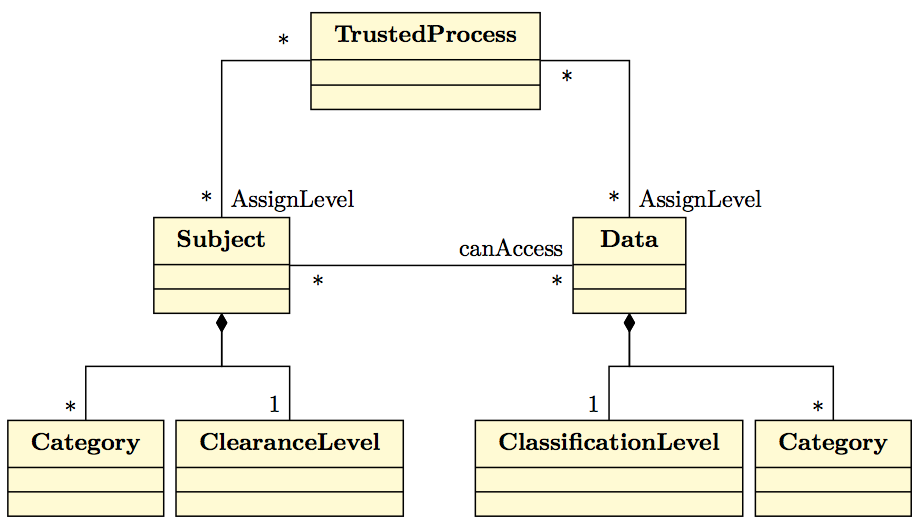
\includegraphics[width=\textwidth]{content/security/accesscontrolmodels/images/multilevelsecurity.png}
\caption{Multilevel Security Klassendiagramm}
\end{figure}

\subsection*{Vorteile}
\begin{itemize}
	\item Welcher Benutzer welche Berechtigung erhalten soll kann relativ einfach am Organigramm einer Organisation abgeleitet werden.
	\item Durch die Modellierung der \emph{Trusted Processes} trennt dieses Pattern strikt zwischen Administration und tatsächliche Umsetzung Sicherheitsregeln.
\end{itemize}

\subsection*{Nachteile}
\begin{itemize}
	\item Bei der Umsetzung dieses Patterns sollte darauf geachtet werden, dass normierte Bezeichnungen für die entsprechenden Sensitivity und Clearance Levels verwendet wird (--> Glossar)
	\item Der \emph{Trusted Process} ist eine kiritsche Stelle im System.\\
	\emph{``Aber wer wird über die Wächter selbst wachen?''}
	\item Daten als auch Benutzer müssen optimalerweise in hierarchische Berechtigungstrukturen eingeteilt werden können.
	Dementsprechend kann dieses Pattern nur schwer auf alltägliche Systeme übertragen werden. (vgl. Militär)
	\item Nur weil ein Subjekt mit einer hohen Sicherheitsklassifizierung ausgestattet wurde, muss dies nicht bedeuten, dass keine Informationen nach Aussen getragen werden.\\Beispiel: Banker telefoniert im Zug lautstark und gibt sensible Kundeninformationen preis.
\end{itemize}

\subsection*{Erweiterungen}
Das Rollenkonzept von \ref{sec:rbac} Role Based Access Control kann mit diesem Pattern problemlos kompiniert werden: Dabei werden die \emph{Clearance Levels} einfach auf die Gruppen statt direkt auf die Benutzer zugwiesen.

\subsection*{Beispielanwendungen}
\begin{itemize}
	\item Militäreisches IT-System
	\item Datenbanksysteme (bspw. Oracle)
	\item Betriebssysteme (bspw. HP Virtual Vault: HP Unix Abkömmling, properitär)
\end{itemize}